\documentclass[beamer]{standalone}

\usepackage{tikz}
\usetikzlibrary{positioning}
\usetikzlibrary{decorations.pathreplacing,decorations.pathmorphing,arrows,fit}
\usetikzlibrary{calc}

\begin{document}

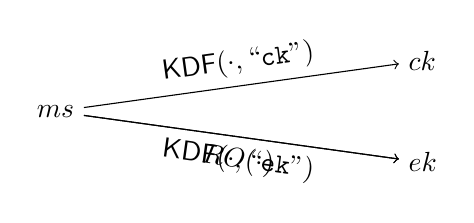
\begin{tikzpicture}

	\node (KDF) {$ms$};
	\node [above right = 0.2 and 4cm of KDF] (ck) {$ck$}; 
	\node [below right = 0.2 and 4cm of KDF] (ek) {$ek$}; 
	
	\draw[->] (KDF) -- node[above,sloped]{$\mathsf{KDF}(\cdot,``\mathtt{ck}")$} (ck);
	\uncover<1-1>{
		\draw[->] (KDF) -- node[below,sloped]{$\mathsf{KDF}(\cdot,``\mathtt{ek}")$} (ek);
	}
	\uncover<2->{
		\draw[->] (KDF) -- node[below,sloped]{$RO(\cdot)$} (ek);
	}
\end{tikzpicture}


\end{document}